\documentclass[12pt]{article}

\usepackage{prilab}
\usepackage{url}

\begin{document}

\maketitle{Lab 02: Information Retrieval Models}

The main goal of this lab is to {\bf implement a simple, memory-based, version of the Vector Space Model for Information Retrieval}, using the Python language.

Your application should take as input a file containing several textual documents, one document per line. The documents should be read from disc and
indexed into memory. Once the documents are stored, the application should read a set of keywords from \emph{stdin} and use it as a query over the indexed
documents. The documents should be presented ordered according to their similarity to the query.

\section{}

Implement a function that reads a file from disc (as described above) and
creates an in-memory \emph{inverted index} of its contents. The efficient construction of disk-based inverted indexes will be covered later on the PRI course and, for now, you should implement a simple in-memory data structure.

The inverted index essentially corresponds to a dictionary that contains, for each term, the documents where it occurs and the corresponding document frequency. The following figure schematically illustrates an inverted index created over a collection of four documents. The figure shows each term, from the vocabulary used in the collection, in association to the documents where the term occurs, and together with the occurrence frequency.

\begin{center}
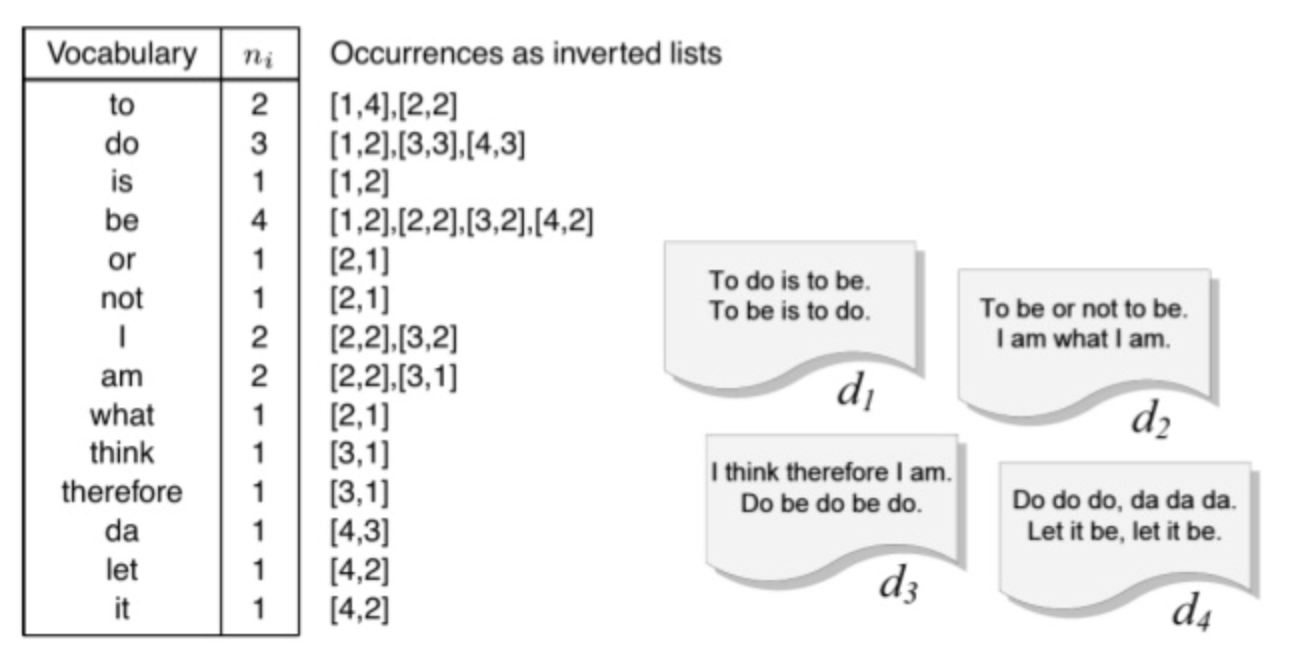
\includegraphics[scale=0.5]{fig-inverted-index}
\end{center}

When reading the file from disk, assume that the terms in each document are separated by any sequence of non-alphanumeric characters. Each document read should be assigned a unique identifier.

\section{}

Using the above function, implement a script to print some statistics on the
documents indexed, namely:
\begin{itemize}
\item The total number of documents;
\item The total number of terms;
\item The total number of individual terms;
\end{itemize}

The script should also take a set of terms as command line arguments and,
for each term, print the following statistics:
\begin{itemize}
\item Document frequency (\emph{DF});
\item Maximum and minimum term frequency (\emph{TF});
\item Inverse Document Frequency(\emph{IDF}), according to the formula $\log(N/DF)$, where $N$ is the total
    number of documents.
\end{itemize}

If needed, change your indexing function so that these values can be easily
obtained (e.g., you can consider indexing the vocabulary used in the document collection, associating each term to the corresponding IDF score, separately from the list that contains the documents where the term occurs, together with the corresponding frequency).

\begin{quote}
    \textbf{Notes:} 

    To read command line arguments in Python, you should use the \texttt{sys.argv} list,
    from the \texttt{sys} module.

    To find the minimum and maximum, try the \texttt{min} and \texttt{max}
    functions.
\end{quote}

\section{}

Implement a function that takes as input a list of terms and computes the
\emph{dot product} similarity between the query formed by those terms and each
indexed document. The function should return a list of pairs (document id,
similarity).

The following pseudo-code shows how this can be implemented efficiently.

\newcommand{\att}{\ensuremath{\leftarrow}}
\newcommand{\fdt}{\ensuremath{TF_{d,t}}}
\begin{itemize}\ttfamily \footnotesize
\item Set $A \att \{\}$
\item For each query term $t \in Q$
    \begin{itemize}
    \item Set $I_t \att$ the inverted list of $t$
    \item Set $idf_t \att \log(N/DF_t)$
    \item For each $(d,\fdt)$ pair in $I_t$
        \begin{itemize}
        \item If $A_d \not\in A$ then
            \begin{itemize}
            \item Set $A_d \att 0$
            \item Set $A \att A \cup \{A_d\}$
            \end{itemize}
        \item Set $A_d \att A_d + \fdt \times idf_t$
        \end{itemize}
    \end{itemize}
\item Return $A$, where each $A_d$ contains the similarity between the query and document $d$.
\end{itemize}

\section{}

With the above functions, create an application that indexes a set of
documents, reads user queries from \emph{stdin}, and produces a list of
documents (or document ids) ordered by their similarity to the query.

\begin{quote}
    \textbf{Note 1:} You can use function \texttt{raw\_input} to read data from
    stdin.
\end{quote}

\begin{quote}
    \textbf{Note 2:} You can test your application with the ``Time'' IR test collection, available from \url{http://ir.dcs.gla.ac.uk/resources/test_collections/time/}
\end{quote}

\section{Pen and Paper Exercise}

Consider the following collection of 4 text documents.

\begin{center}
\tt
\begin{tabular}{ l r }
number & text document \\
\hline
\hline
1 & shipment of gold damaged in fire \\ \hline
2 & delivery of silver arrived in silver truck \\ \hline
3 & shipment of silver arrived in truck \\ \hline
4 & truck damaged in fire \\ \hline
\end{tabular}
\end{center}

Calculate the representations for the documents in the collection according to the Vector Space Model, using TF-IDF weights for the different terms. The TF-IDF score of a term $t$ in a document $d$ from a collection $D$ can be computed through the following equation:

\begin{center}
\begin{equation*}
\mathrm{TF-IDF}(t, d) = \mathrm{frequency}(t,d) \times \log \left( \frac{|D|}{|\{d' \in D: t \in d'\}|} \right)
\end{equation*}
\end{center}

According to the vector space model and using the document representations (i.e., computing the cosine similarity towards the document vectors), find which document in the collection is the most relevant to the following query: {\tt silver truck}. 

\begin{quote}
    \textbf{Note 1:} For simplification, the TF-IDF formula above is not considering the normalization of the TF component with basis on the occurrence frequency of the most frequent term in the document, as shown in the corresponding lecture.
    
    \textbf{Note 2:} After completing the exercise, considering the same user query, you can also experiment with the application of other retrieval models. These include:
    \begin{itemize}
    \item The simple Binary Independence Model (BIM) considering the blind assumptions for $P(k_i|R)$ and $P(k_i|R)$.
    \item The Okapi BM25 model, considering a simple estimate for the IDF component and with $b=0.75$ and $k_1=1.2$.
    \item A simple unigram language modeling approach, without considering parameter smoothing.
    \end{itemize}
    The corresponding equations are given below.
    
    \begin{center}
    \begin{equation*}
{ {\text{BM25}}(q,d)=\sum _{i=1}^{|q|}{\text{IDF}}(q_{i})\cdot {\frac {f(q_{i},d)\cdot (k_{1}+1)}{f(q_{i},d)+k_{1}\cdot \left(1-b+b\cdot {\frac {|d|}{\text{avgdl}}}\right)}},}
    \end{equation*}
    \end{center}
    
\end{quote}

\end{document}
